
\chapter{Crawl.js} % Main chapter title
In this chapter we describe how crawl.js splits and distributes the work in detail.
\label{Chapter4} 
\lhead{Chapter 4. \emph{Crawl.js}} 

\section{System overview}
Crawl.js is a decentralized system. Each \emph{worker} in the system is standalone and autonomous and does not depend on any other worker. The only thing a worker needs is a connection to the \emph{Queues} and the \emph{Stores}. Figure~\ref{system_overview} gives an overview of the main components in the system.

\begin{figure}[h]
\centering
  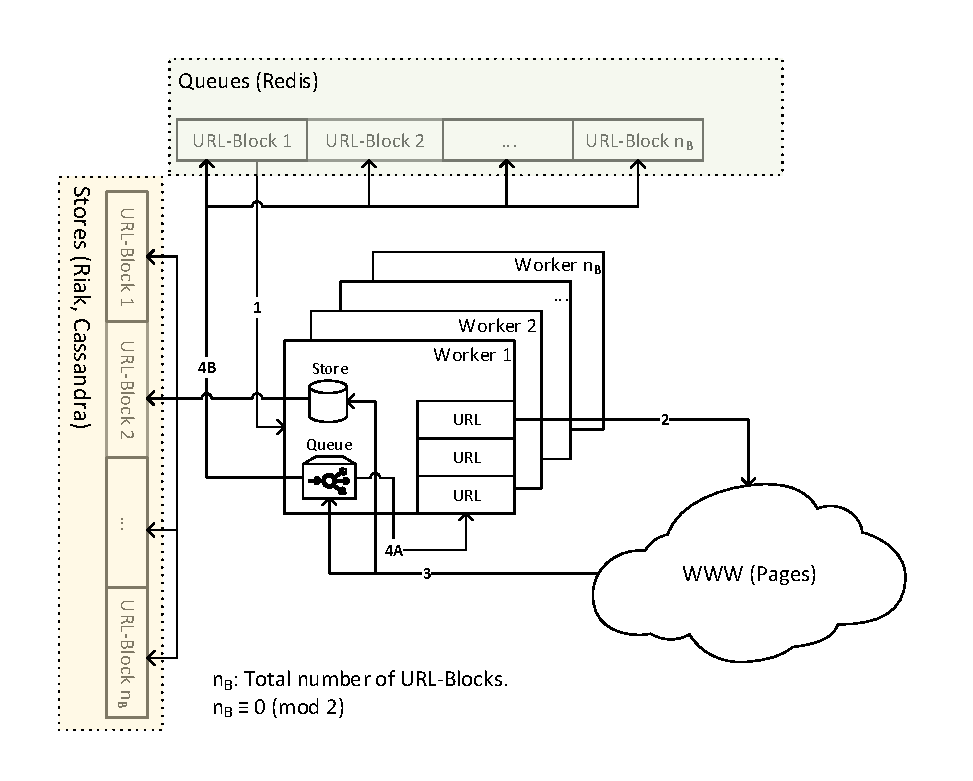
\includegraphics[width=1\textwidth]{Figures/system_overview.pdf}
\caption{Crawl.js - System Overview}
\label{system_overview}
\end{figure}

\subsection{dQueue (A distributed Queue)}
\subsection{URL-Block}
A URL-Block is nothing more than a set of URLs or to be more precise a queue of URLs. It is obvious that at some point we will need some ordering within the set of URLs.
This queue or URL-Block is the entity used to distribute the work. There is always only one consumer (worker) per URL-Block.
This fact of a 1:1 association between a URL-Block and a worker (consumer) is a design choice and we will discuss the dis-/advantages later.

\subsection{Mapper}
Bla bli

\subsection{Worker}
A worker is autonomous and responsible for one URL-Block. Why autonomous? Because a worker can fetch pages, store them and extract new URLs out of it. Newly found URLs are assigned (\emph{Mapper}) to their URL-Block and dispatched automatically. All this happens without any interaction to other components in the system. This keeps the number of inter-communication messages very low.

One worker for one URL-Block. This is true for consuming URLs but obviously we have multiple URL producers. Namely each worker in the system is a candidate for producing new URLs because each one is able to assign and dispatch newly found URLs independly. So we have one consumer and multiple producers whithin one URL-Block (queue).

\subsection{Sponge}
The storage has two main roles in the system. The first is the classic, well-known role of making the downloaded content persistent (html, images, css). The second role of the storage is to provide a persistence layer for the URL-Blocks (queues) described earlier.
There are distinct requirements for the two roles of the storage that we will present later.

\section{dQueues (distributed Queues)}
\subsection{URL-Block (a single Queue)}
\subsection{Implementation (Redis.io)}

\section{Storage}
\subsection{Implementation (Riak)}

\section{Mapper}
\subsection{Requirements}
\subsection{Static mapping}
\subsection{Dynamic mapping}
\subsection{Load-Balancing}

\section{Worker (a crawl.js instance)}
\subsection{States}
Dummy
\subsection{Software Architecture}
Dummy
\subsection{Configuration}
Dummy
\subsection{github}
Dummy
\subsection{Performance}
Dummy
\subsection{Storage}
Dummy
\subsection{Details - (Url-normalization, ..)}

